\documentclass{article}
\usepackage{tikz}
\usepackage[margin=1in]{geometry}
\usetikzlibrary{positioning}
\usetikzlibrary{shapes, arrows}
\begin{document}


\centerline{\sc \large Phase Two Capstone Writeup}
\vspace{.5pc}

\begin{flushleft}
\textbf{Name:} Joshua Abraham
\vspace{.5pc}

\textbf{Date:} 21 SEP 2017
\vspace{.5pc}

\textbf{Current Module:} Phase Two Capstone
\vspace{.5pc}

\textbf{Project Name:} "Mining"
\vspace{.5pc}

\textbf{Project Goals:}
\vspace{.5pc}
\end{flushleft}

This project was quite large and involved many modules, classes, and unit
tests to create a package that implements an Overlord and Drones to mine
minerals from a map. The Overlord and it's drones operate in a simulation
that uses 'ticks' to denote discrete units of time. The simulation begins
with a limited number of 'refined minerals' which are used to spawn Drones,
who scout and mine the map.

\begin{flushleft}
\textbf{Considerations:}
\vspace{.5pc}
\end{flushleft}

\begin{itemize}
	\item[$\bullet$] The project should make use of concepts learned during
	phase two.
	\item[$\bullet$] The 'mining' package must instantiate an Overlord and
	at least two subclasses of Drone.
	\item[$\bullet$] All Zerg units must have health (minimum of 1) and an
	action method that takes a map context as a parameter.
	\item[$\bullet$] All code in the package must follow the PEP8 guidelines.
	\item[$\bullet$] No work should be performed in the 'master' branch.
	\item[$\bullet$] The Overlord class has 1 second to perform it's action
	method, while the Drones have 1 millisecond.
\end{itemize}

\begin{flushleft}
\textbf{Initial Design:}
\vspace{.5pc}
\end{flushleft}

The project is a Python package, composed of several modules and tests:
\begin{itemize}
	\item [$\cdot$] \textit{area.py}: This module contains the Area class
	that is used by drones to represent their view of their map.
	\item [$\cdot$] \textit{dashboard.py}: This module contains the
	Dashboard class that represents all three maps in the simulation.
	\item [$\cdot$] \textit{overlord.py}: This module contains the
	Overlord class that is responsible for creating, deploying, and 
	returning Drones. The Overlord also commands Drones to mine minerals.
	\item [$\cdot$] \textit{drone/}: This directory contains the drone and 
	location modules.
	\item [$\cdot$] \textit{drone.py}: This file contains the Drone, Scout,
	and Miner classes of drone units. 
	\item [$\cdot$] \textit{location.py}: This file contains the Location
	class, which is used by drones to store their current and adjacent 
	tiles.
	\item [$\cdot$] \textit{path.py}: This file contains functions used by
	the Overlord and Drone classes during pathfinding.
	\item [$\cdot$] \textit{zerg.py}: This file contains the abstract class
	Zerg from which Drones and Overlord inherit from.
	\item [$\cdot$] \textit{tests/}: This directory contains unit tests for
	the package.
	\item [$\cdot$] \textit{runtest.sh + runlinter.sh}: These are bash
	scripts to run unit tests and the pep8 linter utility.
\end{itemize}
\vspace{5mm}

\begin{flushleft}
\textbf{Data Flow:}
\vspace{.5pc}
\end{flushleft}

\begin{center}
\begin{equation}
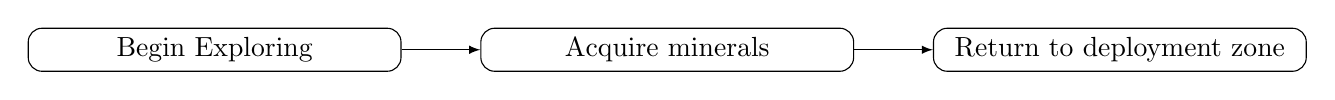
\begin{tikzpicture}[auto, node distance=1cm]
    \tikzstyle{block} = [draw, rectangle];
    \tikzstyle{decision} = [diamond, draw, fill=blue!20, 
    text width=4.5em, text badly centered, node distance=2cm, inner sep=0pt]
    \tikzstyle{rblock}=[draw, shape=rectangle,rounded corners=0.5em,
    text width=4.5cm, align=center];
    \tikzstyle{line}=[-latex];
    \node [rblock] (a) {Begin Exploring};
    \node [rblock,right=of a] (b) {Acquire minerals};
    \node [rblock,right=of b] (c) {Return to deployment zone};
    \draw[line] (a) -- (b);
    \draw[line] (b) -- (c);
\end{tikzpicture}
\end{equation}
\end{center}
\vspace{5mm}

The Overlord spawns the Drones that it can afford with it's refined 
minerals.  These Drones are then deployed to each map and begin exploring.
Drones explore by following a simple set of rules: if an adjacent tile is
both unexplored and passable, it will move there. Each time a Drone moves
it updates it's internal representation of the map. When the drone is
finished exploring it sets a flag that signals it is ready to mine.  The 
Overlord polls every deployed Drone and monitors the status of their flags.
When a Drone signals it is ready to mine, the Overlord converts the Drone's
map into an adjacency list and performs a breadth-first-search to generate 
a path to a mineral field to mine.  The Overlord gives this path to the 
Drone, who carries them out. This process repeats until the Drone's 
carrying capacity is depleted.  The Drone then generates a path back to the
deployment zone and returns home.  The Drone sets it's returning flag and
when the Overlord sees this flag, it returns the unit.

\begin{flushleft}
\textbf{Communications Protocol:}
\vspace{.5pc}
\end{flushleft}

The Overlord and Drones "communicated" via setting attributes.  No other 
communications were used in this project.

\begin{flushleft}
\textbf{Potential Pitfalls:}
\vspace{.5pc}
\end{flushleft}

\begin{itemize}
	\item[$\bullet$] Having too much logic in the Drone and causing 
	timeouts.
	\item[$\bullet$] Deeply nested if..else statements for path decision
	making. (Especially for readability)
	\item[$\bullet$] 
\end{itemize}

\begin{flushleft}
\textbf{Test Plan:}
\vspace{.5pc}
\end{flushleft}

\textit{User Tests:}
\begin{itemize}
	\item[$\cdot$] Use the started code provided by instructor to "drive"
	package.
	\item[$\cdot$] Run the \textit{world.py} starter file with various
	values for ticks, and refined minerals.
	\item[$\cdot$] 
\end{itemize}

\textit{Test Cases:}
\begin{itemize}
	\item[$\cdot$] Unit tests for every class and method. (where feasibly 
	posible)
	\item[$\cdot$] Test inter-object communication.
	\item[$\cdot$] 
\end{itemize}

\begin{flushleft}
\textbf{Conclusion:}
\vspace{.5pc}
\end{flushleft}


\begin{center}
\begin{equation}
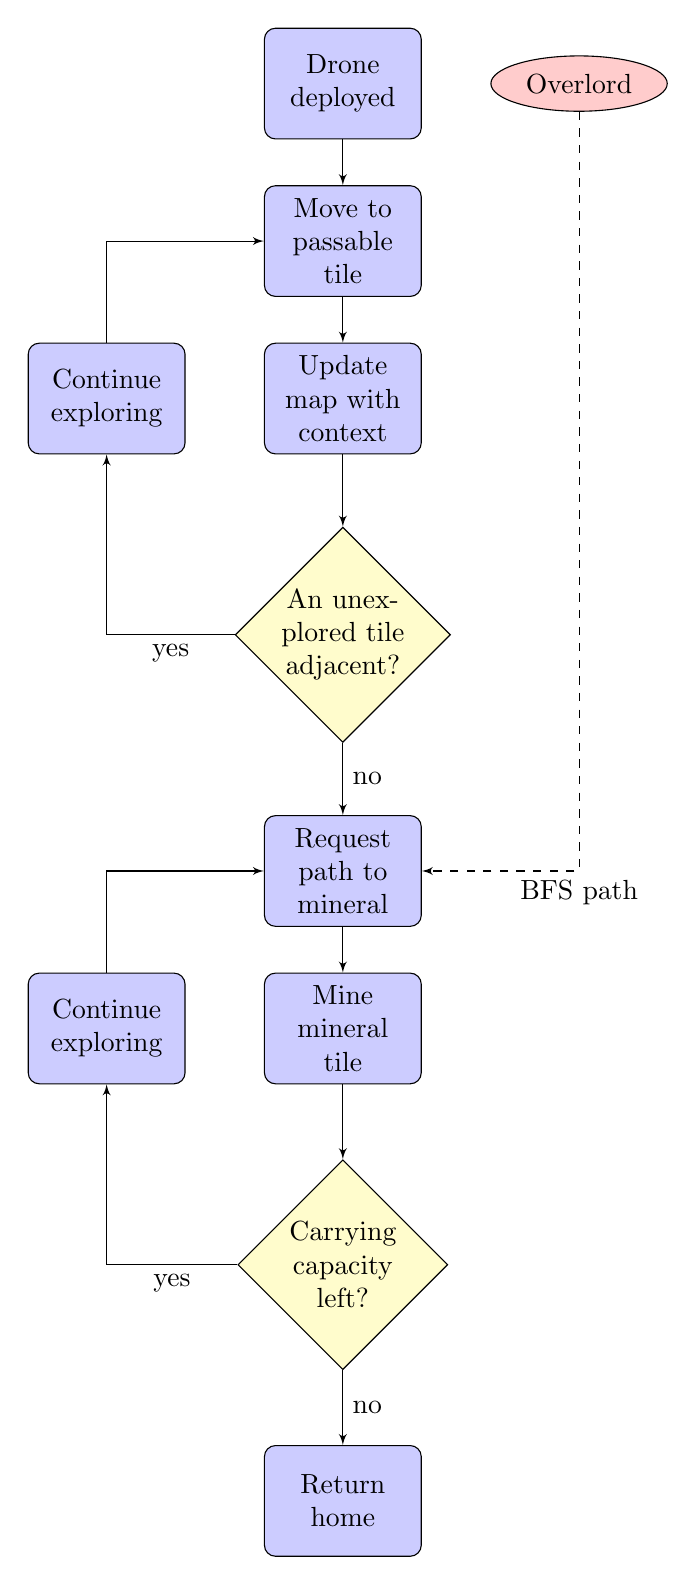
\begin{tikzpicture}[node distance = 2cm, auto]
    \tikzstyle{decision} = [diamond, draw, fill=yellow!20, 
    text width=4.5em, text badly centered, node distance=3cm, inner sep=0pt]
    \tikzstyle{block} = [rectangle, draw, fill=blue!20, 
    text width=5em, text centered, rounded corners, minimum height=4em]
    \tikzstyle{line} = [draw, -latex']
    \tikzstyle{cloud} = [draw, ellipse,fill=red!20, node distance=3cm,
    minimum height=2em]
    \node [block] (deploy) {Drone deployed};
    \node [cloud, right of=deploy] (overlord) {Overlord};
    \node [block, below of=deploy] (identify) {Move to passable tile};
    \node [block, below of=identify] (evaluate) {Update map with context};
    \node [block, left of=evaluate, node distance=3cm] (update) {Continue 
    exploring};
    \node [decision, below of=evaluate] (decide) {An unexplored tile 
    adjacent?};
    \node [block, below of=decide, node distance=3cm] (request) {Request path
    to mineral};
    \node [block, below of=request] (minepath) {Mine 
    mineral tile};
    \node [decision, below of=minepath] (keepmining) {Carrying capacity
    left?};
    \node [block, left of=minepath, node distance=3cm] (anotherpath)
    {Continue exploring};
    \node [block, below of=keepmining, node distance=3cm] (return) {Return home};
    \path [line] (deploy) -- (identify);
    \path [line] (identify) -- (evaluate);
    \path [line] (evaluate) -- (decide);
    \path [line] (request) -- (minepath);
    \path [line] (minepath) -- (keepmining);
    \path [line] (decide) -| node [near start] {yes} (update);
    \path [line] (update) |- (identify);
    \path [line] (decide) -- node {no}(request);
    \path [line,dashed] (overlord) |- node [midway,below] {BFS path} 
    (request);
    \path [line] (keepmining) -| node [near start] {yes} (anotherpath);
    \path [line] (anotherpath) |- (request);
    \path [line] (keepmining) -- node {no}(return);
\end{tikzpicture}
\end{equation}
\end{center}

\end{document}